\section{Simulating the Ising Model}
Now we will look to simulate the two dimensional Ising spin model on an $(L \times L)$ square lattice.	The total energy of the system is 
\begin{equation}
\frac{1}{2}\sum_{i=0}^{L-1}\sum_{j=0}^{L-1}E_{i,j}
\end{equation}
with
\begin{equation}
E_{i,j} = -\sigma_{i,j}(\sigma_{i+1,j} + \sigma_{i-1,j} + \sigma_{i,j+1} + \sigma_{i,j-1}).
\end{equation}
Spins can take the values $\pm 1$ and we use periodic boundary conditions.

The observables we are interested in are the energy density
\begin{equation}
e =\left \langle \frac{E}{L^2}\right\rangle
\end{equation}
and the magnetization density
\begin{equation}
m = \langle |\mu| \rangle
\end{equation}
\begin{equation}
\mu = \frac{1}{L^2} \sum_{i=0}^{L-1}\sum_{j=0}^{L-1}\sigma_{i,j}
\end{equation}

The measurement of the total energy $E$ and magnetization density $\langle\mu\rangle$ for a given state are implemented as
\listfile{../src/ising_lib.py}{src/ising\_lib.py}{16}{31}{Observable Measurement}{observe}
\subsection{Exact Summation}
We begin by computing the expectation values of these two observables directly from the partition function. This is possible if we use a box size of $L=4$ which we will use for the rest of the worksheet. Expectation values of observables can be calculated by
\begin{equation}
\left\langle A \right\rangle = \frac{\sum_\Phi A_\phi e^{-E_\phi /T}}{\sum_\Phi e^{-E_\phi /T}}.
\label{eq:part}
\end{equation}
In order to calculate this sum we need to generate every possible state of the finite 2D Ising system. We do this by counting to $2^{16}$ in binary. All the necessary states are represented by all of the 16 digit binary numbers. We simply replace $0$ with $-1$ and map back onto a square lattice. The following function performs the neccesary generation.
\listfile{../src/ising_lib.py}{src/ising\_lib.py}{44}{56}{State Generation}{states}

Equipped with the set of states, we are prepared to calculate the sum in \ref{eq:part} for various temperatures $T = {1.0, 1.1, ..., 4.9, 5.0}$. This is accomplished for our observables of interest with the next code block.
\listfile{../src/ising_exact.py}{src/ising\_exact.py}{6}{16}{Exact Summation}{exact}

The blue curve in figures \ref{fig:ising_e} and \ref{fig:ising_m} show the expectaion values of our two observables due to exact summation.
\subsection{Monte Carlo}
The exact calculation in the preceding section is quite slow and will not withstand a simulation with more spins so we will use Monte Carlo simulation to obtain the same information. We will use the Metropolis-Hastings algorithm to select states. One Monte Carlo step is implemented as follows.
\listfile{../src/ising_lib.py}{src/ising\_lib.py}{33}{42}{Monte Carlo Step}{isingmc}
We then run $10000$ MC steps for each of our previously listed temperatures.
\listfile{../src/ising_mc.py}{src/ising\_mc.py}{5}{15}{MC Simulation}{isingmcdat}
The points in figures \ref{fig:ising_e} and \ref{fig:ising_m} show the values of magnetization and energy density measured via Monte Carlo.
\subsection{Error Analysis}
Since each step in our simulation is derived from the previous one, the data is obviously correlated and we can't use the obvious method for estimating error. In this case we will use binning analysis. This involves breaking our time series into $N_B$ bins. If the bin length $k$ is large enough then these bins will be uncorrelated. Clearly $\bar{O}_B = \bar{O}$ and we can calculate the squared error as
\begin{equation}
\epsilon^2_{\bar{O}} = \frac{1}{N_B(N_B-1))}\sum_{n=1}^{N_B}(O_{B,n} - \bar{O})^2,
\end{equation}
correlation time as
\begin{equation}
\tau = \frac{k \epsilon^2_{\bar{O}}}{2 N \sigma^2_{O_i}},
\end{equation}
and effective sample size as 
\begin{equation}
N_{\mathrm{eff}} = N/2\tau
\end{equation}
In order to take care of the free parameter k, we perform the entire error analysis with $1 \leq k \leq N/10$ and take the highest autocorrelation time.
\listfile{../src/ising_lib.py}{src/ising\_lib.py}{65}{93}{Error Analysis}{error}

In order to test our error analysis we will calculate statistics about a bivariate Gaussian. We use the following function to generate samples from a bivariate Gaussian.
\listfile{../src/ising_lib.py}{src/ising\_lib.py}{58}{63}{Bivariate Gaussian}{gauss}
We choose $N = 1e6$ and $\rho = 0.99005$ and the autocorrelation time is known to be
\begin{equation}
\tau = \frac{1}{2}\frac{1+\rho}{1-\rho} \approx 100.003
\end{equation}
Using our error\_analysis function we find
\begin{equation}
\bar{O}=-0.0054, \quad k = 15625, \quad \tau = 104.2, \quad N_\mathrm{eff} = 4699.6, \quad \epsilon^2_{\bar{O}} = 0.0143
\end{equation}
Finally we use our analysis program to calculate the error in the MC measurements of energy and magnetization density.
\begin{figure}[ht]
	\centering
	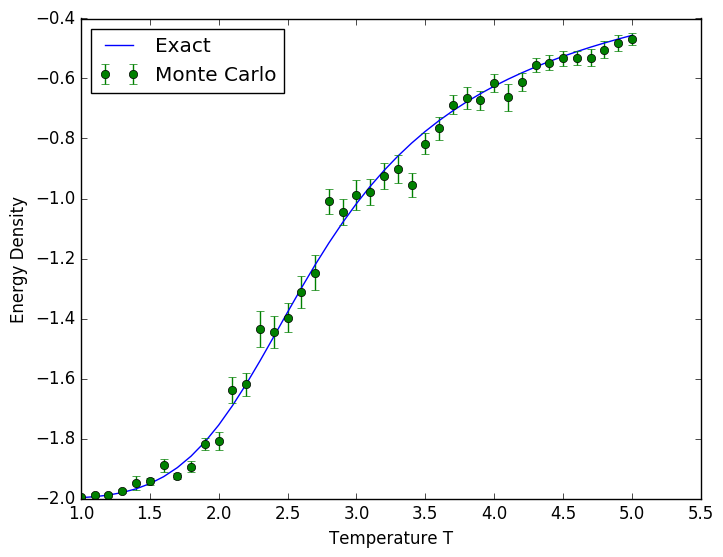
\includegraphics[width=0.7\textwidth]{../fig/errorplot_e.png}
	\caption{
		Energy density of our 2D Ising spin system as a function of temperature. The blue curve is due to exact summation and the points refer to the Monte Carlo algorithm. Error bars are calculated using binning analysis.}
	\label{fig:ising_e}
\end{figure}
\begin{figure}[ht]
	\centering
	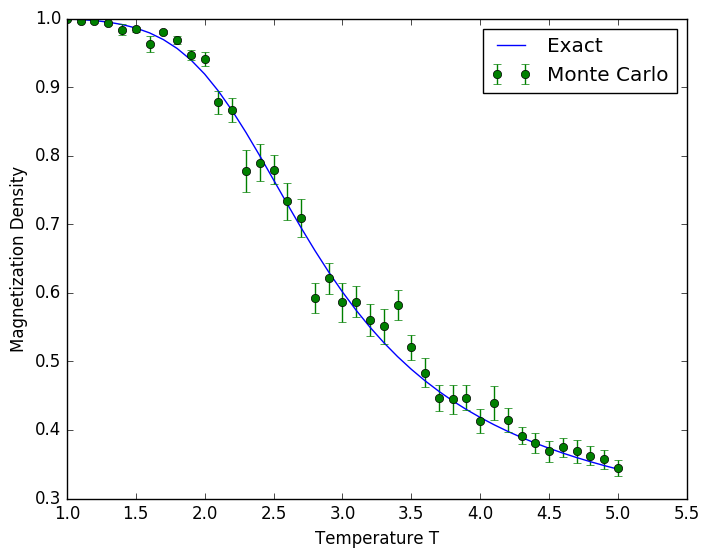
\includegraphics[width=0.7\textwidth]{../fig/errorplot_m.png}
	\caption{
		Magnetization density of our 2D Ising spin system as a function of temperature. The blue curve is due to exact summation and the points refer to the Monte Carlo algorithm. Error bars are calculated using binning analysis.}
	\label{fig:ising_m}
\end{figure}